\subsection{Tonhöhenverarbeitung}\label{subsec:Pitch_Generation}

Die Hauptaufgabe der Komponente \textit{Tonhöhenverarbeitung} ist es das Audiosignal aus dem Rechtecksignal des Tonhöhenoszillators zu generieren. Die \textit{Tonhöhenverarbeitung} nimmt zudem eine Frequenzmessung des Audiosignals vor um diverse Funktionalitäten zu gewährleisten. In Abbildung \ref{img:Blockschaltbild_pitch} ist der Grobe Aufbau der Komponente aufgezeigt. Die genaue Erklärung zu den einzelnen Komponenten ist in den folgenden Abschnitten zu finden.


\begin{figure}[h!]
	\centering
	\includegraphics[width=\textwidth]{Blockschaltbild_pitch.pdf}
	\caption{Blockschaltbild der Custom IP \textit{Tonhöhenverarbeitung}} 
	\label{img:Blockschaltbild_pitch}
\end{figure}  



\paragraph{Referenzoszillator}\mbox{}\\

Der \textit{Referenzoszillator} ist wie in der analogen Version aus Kapitel \ref{subsec:Theremin_analog} dafür zuständig ein Sinussignal mit einer Frequenz nahe der des Tonhöhenoszillators zu generieren und an \textit{ref\_out} auszugeben. Er generiert diesen wie schon erwähnt mithilfe des Cordic Algorithmus. Er ist aufgeteilt in zwei Komponenten: der \textit{Cordic Prozessor} und der \textit{Cordic Controller}. Wie diese beiden Komponenten miteinander verbunden sind ist in Abbildung \ref{img:Referenceoscillator} ersichtlich. Beide Komponenten stammen aus dem Projekt 5. Änderungen, welche im Projekt 6 stattfanden, sind entsprechend gekennzeichnet. \\

\begin{figure}[t]
	\centering
	\includegraphics[width=0.53\textwidth]{Referenceoscillator.pdf}
	\caption{Aufbau des Referenzoszillators} 
	\label{img:Referenceoscillator}
\end{figure}  

Der \textit{Cordic Prozessor} ist die eigentliche Implementierung des Cordic Algorithmus wie er in Kapitel \ref{subsec:Cordic} beschrieben wurde. Er muss jedoch für den Einsatz im FPGA leicht angepasst werden. \\
Die Berechnung der Werte für \(\arctan{2^{-i}}\) fand vorgängig statt und ist in eine Lookup Table gespeichert. Dies spart Ressourcen für diese komplizierte Berechnung ein. Wir haben uns entschieden den Algorithmus in einer Pipeline zu implementieren. Dies führt einerseits zu einer höheren maximalen Clockfrequenz, andererseits aber auch zu einer grösseren Signallatenz. Dies ist jedoch nicht problematisch für die gewählte Anwendung, da die Latenz im Nanosekundenbereich ist und später nicht hörbar auffällt. Zuletzt ist eine Multiplikation mit \(2^{-i}\) ganz einfach durch eine Verschiebung um \(i\) Bits nach rechts ersetzbar. Dies spart wiederum Ressourcen ein.\\
Das berechnete Resultat ist als signed Zahl definiert um die Berechnung von negativen Zahlen zu ermöglichen. Sie sind im fixed-point Format und haben \SI{16}{Bit} Länge. Dabei sind von den \SI{16}{Bit} \SI{1}{Bit} Vorzeichen und \SI{15}{Bit} Nachkommastellen. Dies entspricht einem Zahlenbereich von -1 bis 0.999969. Die berechneten Werte gibt der \textit{Cordic Prozessor} an \textit{ref\_out} aus.

Für die Berechnung der Sinuswerte muss ein Winkelwert berechnet werden, der mit der Zeit so ändert, dass sich am Ausgang des Cordic Prozessor ein Sinus mit der gewünschten Frequenz ergibt. Der berechnete Winkelwert wird an \textit{phi} ausgegeben. Für diese Aufgabe ist der \textit{Cordic Controller} zuständig. Bei mit der Zeit linear ansteigendem Winkelwert ergibt sich am Ausgang die gewünschte Sinusform. Wichtig ist jedoch, dass der Cordic Algorithmus nur für Winkelwerte zwischen \(-\pi/2\) und \(\pi/2\) oder anders für Werte im ersten und zweiten Quadranten konvergiert. Die Lösung für dieses Problem ist in Abbildung \ref{img:Cordic_phi} ersichtlich. 
Als erstes wird der Sägezahn Winkel berechnet. Für den linearen Anstieg des Winkels zählt der \textit{Cordic Controller} einen Zähler mit einer bestimmten Schrittweite jeden Clockzyklus hoch. Der wrap-around des Zählers ist dabei erwünscht um den Sprung zwischen dem II und III Quadranten zu erzielen. Der Schrittwert ergibt sich wie folgt:

\begin{equation}
step = \frac{2^{n+1}f_{sig}}{f_{clk}}
\label{equ:cordic_step}
\end{equation} 

Wobei \(n\) die Anzahl Bits des Wertebereichs des Dreiecks Winkels ist, \(f_{sig}\) die gewünschte Frequenz des generierten Signals und \(f_{clk}\) die Clock Frequenz des FPGA.

Nun kommt die bereits erwähnte Einschränkung des Cordic Algorithmus ins Spiel. Die berechneten Werte des Sägezahnwinkels zwischen dem II und III Quadranten konvergieren nicht. Aus diesem Grund konvertiert der \textit{Cordic Controller} diesen Winkel in den Dreieckswinkel. Sind die beiden vordersten Bits entweder \(01\) oder \(10\) befindet sich der Winkelwert im II respektive III Quadranten. Um in diesem Fall den Dreieckswinkel zu erhalten invertiert der \textit{Cordic Controller} alle Bits ausser dem most-significant Bit. Wie man sich leicht davon überzeugen kann ergibt der Dreieckswinkel denselben Sinusverlauf wie der Sägezahnwinkel bei einer Sinusrechnung ohne die erwähnten Einschränkungen. \cite{Cordic}

Um die Kalibrierung und den Glissandoeffekt für das Theremin zu ermöglichen waren im Projekt 6 kleine Anpassungen am \textit{Cordic Controller} nötig. Wie zuvor hat der Controller eine fixe Frequenz implementiert, welche in der Grössenordnung \SI{550}{kHz} liegt. Jedoch legt die Frequenzmessungskomponente nun eine Differenz über einen Eingang an den Cordic Controller an um die zuvor genannten Features über den Referenzoszillator zu ermöglichen.


\begin{figure}[t]
	\centering
	\includegraphics[width=0.8\textwidth]{Cordic_phi.pdf}
	\caption{berechneter Winkel \textit{phi} des Cordic Controllers in Funktion der Zeit} 
	\label{img:Cordic_phi}
\end{figure}  


\paragraph{Mischer}\mbox{}\\

Die Implementation des \textit{Mischers} ist dank der Entscheidung für die Rechteckform des Tonhöhenoszillatorsignals sehr einfach. Über einen GPIO liest der Mischer das Signal des Tonhöhenoszillators ein und verrechnet es mit dem generierten Sinus \textit{ref\_out}. Eine \textit{1} des Rechtecks wird dabei als die Zahl \textit{1} und eine \textit{0} als die Zahl \textit{-1} interpretiert. Die Multiplikation zwischen der \textit{1} und \textit{ref\_out} ist dabei nicht nötig und eine Multiplikation mit \textit{-1} erzielt der Mischer durch das Bilden des Zweierkomplement von \textit{ref\_out}.

\paragraph{Filter}\mbox{}\\

Im Projekt 5 war das \textit{Filter} ein einzelnes CIC-Filter mit dem Dezimationsfaktor 1000. Dies hatte zur Folge, dass viel Aliasing entstand. Um dieses zu verringern haben wir uns im Projekt 6 für den Aufbau aus Abbildung \ref{img:Filter_Pitch} entschieden. Die drei Filter CIC 1 bis CIC 3 sind Instanzen einer CIC-Filter Komponente. Diese Komponente stammt weitestgehend aus dem Projekt 5, ist jedoch auf mehr Modularität erweitert. Die Parameter der drei Instanzen sind in Tabelle \ref{tab:cic_pitch} ersichtlich. Da es bei CIC-Filtern wie in Kapitel \ref{subsec:CIC_Filter} beschrieben, um deren Nullstellen zu Aliasing kommt, sind diese Filter so eingestellt, dass sich die Oberwellen des Rechteck möglichst nicht in deren Nähe befinden. Bei \textit{CIC 1} wurde eine höhere Ordnung gewählt um am Anfang eine stärkere Dämpfung zu erzielen. Die Anzahl Ausgangsbits erhält man mit Formel \ref{equ:cic_bitgrowth} in Kapitel \ref{subsec:CIC_Filter}.\\
Zuletzt haben wir noch ein FIR-Filter implementiert um das Signal auf 48kHz unter abzutasten. Das Filter hat eine Passfrequenz von \SI{2}{kHz} und eine Stopfrequenz von \SI{24}{kHz} mit einer Dämpfung von 55dB. Wir entschieden uns die Koeffizienten mit dem \textit{filterDesigner Tool} von Matlab zu berechnen und als \SI{27}{Bit} signed Zahlen in einer Lookup Table zu speichern. Wir wählten deshalb \SI{27}{Bit}, da im FPGA eine solche Multiplikation noch knapp in einen DSP Block integriert werden kann. \cite{Cyclone_V}
Weswegen der Ausgang Frequenzmessung nach dem zweiten CIC-Filter gewählt wurde ist in einem späteren Abschnitt beschrieben.


\begin{figure}[t]
	\centering
	\includegraphics[width=1\textwidth]{Filter_pitch.pdf}
	\caption{Aufbau des Filters in der Komponente Pitch Generation} 
	\label{img:Filter_Pitch}
\end{figure}  

\begin{table}[t]
	\centering
	\caption{Parameter der drei CIC-Filter}
	\label{tab:cic_pitch}
	\begin{tabular}{l|l|l|l|l}
		\textbf{Komponente} & \textbf{Dezim.Fakt.} & \textbf{Ordnung} &  \textbf{Ausgangsfreq.} & \textbf{Ausgangsbits}\\
		\hline\hline
		CIC 1 & 5 & 2 & \SI{10.8}{MHz} & \SI{21}{Bits}  \\ \hline
		CIC 2 & 9 & 1  & \SI{12}{MHz} & \SI{25}{Bits}  \\ \hline
		CIC 3 & 5 & 1 & \SI{240}{kHz} & \SI{28}{Bits}  \\ \hline	
	\end{tabular}
\end{table}

\paragraph{Verstärker}\mbox{}\\

Die Komponente \textit{Verstärker} ist dafür zuständig beim Signal \textit{filt\_out} den Gain der CIC-Filter zu kompensieren und anschliessend dieses mit der Dämpfung, welche die Lautstärkeverarbeitung liefert, zu multiplizieren. In Abbildung \ref{img:Zero_Cross} ist eine Problematik aufgezeigt, welche auftritt, wenn man die Dämpfung zu beliebigen Zeiten wechselt. Links ist zu sehe, was passiert, wenn die Dämpfung beim höchsten Wert der positiven Halbwelle ändert. Diese Sprünge im Signal treten dann als hörbares Knacksen auf. Um dies zu verhindern ist eine Erkennung von Nulldurchgängen implementiert, dass wie in der Abbildung rechts die Dämpfungen nur bei diesen Nullstellen ändern. Da der Codec ein offsetbehaftetes Signal verlangt muss das most-significant Bit des Signal getoggelt werden um dies zu bewerkstelligen. Diese Komponente enthält zudem die Kommunikation mit dem Streaming Interface. \\
Die Dämpfung des Audiosignals könnte auch über den Codec gemacht werden. Weshalb dies nicht möglich ist, ist in Kapitel \ref{subsec:audio} beschrieben. 
	
\begin{figure}[h!]
	\centering
	\includegraphics[width=1\textwidth]{Zero_Cross.pdf}
	\caption{Unterschied Dämpfungswechsel (links ohne und rechts mit Nullstellenerkennung)} 
	\label{img:Zero_Cross}
\end{figure}  

\newpage

\paragraph{Frequenzmessung, Kalibration \& Glissandoeffekt}\mbox{}\\

Die Komponente \textit{Frequenzmessung} hat mehrere Aufgaben und ist diejenige Komponente mit welcher über den Nios II Prozessor die gesamte \textit{Tonhöhenverabreitung} gesteuert werden kann. Der Aufbau dieser Komponente ist in Abbildung \ref{img:freq_meas_pitch} aufgezeigt.\\
Zum einen wird hier die Frequenzmessung durchgeführt. Dies geschieht über die drei Komponenten FIR, Periodenzähler und Goldschmidtdividierer. FIR ist wie der Name sagt ein FIR Filter. Dieses ist nötig um das Signal aus den CIC-Filtern, welches noch hochfrequente Anteile enthält zu filtern. Das FIR Filter hat eine Passfrequenz von \SI{2}{kHz} eine Stopfrequenz von \SI{40}{kHz} und eine Dämpfung von 30dB. Das Filter ist mit dem \textit{filterDesigner} Tool in Matlab berechnet. Wir haben entschieden die Filterkoeffizienten als fixed-point signed Zahlen in einem Array mit \SI{18}{bit} länge abzuspeichern. Auf dieser Koeffizientenlänge kann Quartus die DSP-Blöcke so nutzen, dass nach der Multiplikation des Signals mit den Koeffizienten die Resultate gleich in den Blöcken addiert wird. Dies ermöglicht längere Multiplikationsketten. \cite{Cyclone_V}\\
Anschliessend wird das Signal \textit{fir\_out} im \textit{Periodenzähler} ausgemessen. Dieser zählt von Nulldurchgang zu Nulldurchgang einen Zähler hoch. Bei einem Nulldurchgang wird der Wert dieses Zählers am Signal \textit{per\_cnt} ausgegeben. Der Zählerwert entspricht der Anzahl Abtastwerte des Signals in einer Signalperiode. \\
Das Signal hat eine Abtastfrequenz von \SI{1.2}{MHz}. Dividiert man diese Abtastfrequenz durch die zuvor gezählte Anzahl Abtastperioden erhält man die Frequenz des Signals.\\ Um diese Division zu berechnen haben wir uns entschieden den Goldschmidt Algorithmus aus Kapitel \ref{subsec:Goldschmidt} einzusetzen. Dieser hat den Vorteil, dass er auch Nachkommastellen berechnen kann um die nötige Genauigkeit bei den tiefen Frequenzen zu erreichen wie in Kapitel \ref{subsec:Musiktheorie} beschrieben. Dass die Berechnungsdauer des Algorithmus nicht für alle Zahlen gleich ist, ist nicht Problematisch, da diese Zeiten im Nanosekundenbereich liegen und nicht hörbar sind. Der Messbereich der Frequenzmessung fängt bei \SI{100}{Hz} an und geht bis \SI{10}{kHz}. Alle Frequenzen darunter oder darüber zeigen \SI{100}{Hz} respektive \SI{10}{kHz} an.

\begin{figure}[h!]
	\centering
	\includegraphics[width=1\textwidth]{freq_meas_pitch.pdf}
	\caption{Aufbau der Frequenzmessung, Kalibration und Glissandoeffekt in der Komponente Pitch Generation} 
	\label{img:freq_meas_pitch}
\end{figure}  

Die gemessene Frequenz wird anschliessend in der Komponente \textit{Kalibration \& Glissando} benötigt. Diese ist dafür zuständig einerseits die Tonhöhe zu kalibrieren und andererseits den Glissando-Effekt zu steuern. Um die Frequenz des Audiosignals für diese Funktionen zu verändern verstimmt die Komponente den Referenzoszillator entsprechenden. Kalibration \& Glissando addiert die Differenz welche den Glissandoeffekt hervorruft und die Änderung welche während der Kalibration berechnet wurde und übergibt das Resultat dem Referenzoszillator. Diese wird von nun an als Frequenzdifferenz bezeichnet. Die Steuerung dieser Funktionen ist als State-Machine aufgebaut wie in Abbildung \ref{img:state_event_Cal_Glis} zu sehen ist. 
Dabei sind die States reset, check, sign und diff für die Kalibration zuständig und freq range, step und step count für den Glissando-Effekt zuständig. Es folgt eine Erklärung, was in den einzelnen Zuständen geschieht:

\textbf{Idle}:
Der Idle State setzt die Frequenzdifferenz auf die berechnete Differenz der Kalibrierung. Der Anteil des Glissando-Effekts wird auf 0Hz gesetzt.

\textbf{reset}:
Der alte Kalibrationswert wird gelöscht und gewartet bis eine neue Frequenzmessung abgeschlossen ist.

\textbf{check}:
Da die Messung Frequenzen unter \SI{100}{Hz} immer als \SI{100}{Hz} angibt, muss die Komponente diese erkennen. Bei einer Messung von \SI{100}{Hz} inkrementiert die Komponente Calibration \& Glissando die Frequenzdifferenz um \SI{400}{Hz}. Dies führt dazu, dass bei der nächsten Messung das Signal nicht mehr in dem Bereich liegt, in dem die Messung immer \SI{100}{Hz} misst.

\textbf{sign}:
Für die in Kapitel \ref{sec:Konzept} beschriebene Spielweise, dass mit kleinerer Distanz zur Antenne die Tonhöhe steigt, ist der State sign zuständig. Ist der Referenzoszillator so eingestellt, dass dessen Frequenz kleiner ist als die des Tonhöhenoszillators, so würde bei Annäherung des Spielers an die Antenne die Frequenz des Audiosignals zuerst sinken, bis die beiden Oszillatorfrequenzen gleich sind. Dies, da die Frequenz des Tonhöhenoszillators mit kleinerem Abstand immer mehr sinkt. Anschliessend würde sie wieder steigen, da der Tonhöhenoszillator kleiner ist als der Referenzoszillator. Um zu erkennen ob dies der Fall ist, subtrahiert die Komponente \SI{100}{Hz} von der Frequenzdifferenz. Ist die nachfolgende Messung grösser geworden, bedeutet dies, dass der Referenzoszillator kleiner war als der Tonhöhenoszillator. Nun kann ganz einfach die gemessene Frequenz verdoppelt und zu der Frequenzdifferenz addiert werden, damit der Referenzoszillator die grössere Frequenz hat.

\textbf{diff}:
Nach den letzten drei States ist nun sichergestellt, dass der Referenzoszillator grösser ist als der Tonhöhenoszillator. Jedoch sollen ja diese beiden Oszillatoren aufeinander abgestimmt sein. Dazu wird abwechslungsweise die Frequenzdifferent um einen kleinen Schritt dekrementiert und danach die Frequenz gemessen. Wir haben uns dafür entschieden, dass wenn die Messung \SI{120}{Hz} unterschreitet die Kalibration abgeschlossen ist. Dies da Töne unterhalb dieser Frequenz sehr merkwürdig klingen.

\textbf{freq range}:
Der State freq range ist dafür zuständig herauszufinden, welcher diskrete Ton der gewählten Tonleiter (normal oder pentatonisch) am nächsten zur gemessenen Frequenz ist. Die Frequenz wird dabei mit einer Lookup-Table mit allen Grenzen zwischen den Tönen verglichen. ist die Frequenz ausserhalb des gewählten Frequenzbereich wird hier abgebrochen und in den State idle gewechselt.

\textbf{step}:
Der State step bestimmt die Schrittgrösse, welcher im nächsten State für die Annäherung nötig ist. Die Schrittgrössen für alle Töne sind im Vorhinein berechnet als \SI{1}{Cent} Differenz zum eigentlichen Ton. Würde überall die gleiche Schrittgrösse genommen, wäre das Aufschliessen bei hohen Tönen extrem langsam und bei tiefen Tönen so schnell, dass kein Übergang hörbar ist. 

\textbf{step count}:
Der letzte State verrechnet die Frequenzdifferenz in vorgegebenen Intervallen mit dem zuvor bestimmten Step, bis auf den Ton aufgeschlossen ist. Hat die Frequenzmessung jedoch während dem Zählen eine neue Frequenz gemessen wird in den State freq range gewechselt. Erreicht das Aufschliessen bevor eine neue Messung stattfand einen Unterschied von unter \SI{6}{Cent} zu der anzunähernden Frequenz, stoppt das Zählen bis zu einer neuen Messung.

\begin{figure}[h!]
	\centering
	\includegraphics[width=1\textwidth]{state_machine_Cal_Glis.pdf}
	\caption{State Event Diagramm der Kalibration \& Glissando Komponente} 
	\label{img:state_event_Cal_Glis}
\end{figure} 

\paragraph{Register}\mbox{}\\
Um mit der Komponente \textit{Tonhöhenverarbeitung} über das Memory-Mapped Interface kommunizieren zu können haben wir folgende Register definiert:

\begin{table}[H]
	\centering
	\caption{Zusammenfassung der Register}
	\label{tab:Registers_pitch}
	\begin{tabular}{l|l|l|l|l|l|l}
		\textbf{Register} & \textbf{Adresse} & \textbf{R/W} &	\multicolumn{4}{l}{\textbf{Bits}} \\\cline{4-7}
						  &					 &				& \textbf{31-3}  & \textbf{2} & \textbf{1} & \textbf{0}\\ 
		\hline \hline
		
		cntrl\_reg & 00 & R/W & X & scale & cal & glis \\ 
		\hline
		freq\_data\_reg & 01 & R & \multicolumn{4}{l}{Frequenz} \\
		\hline
		delay\_data\_reg & 10 & W & \multicolumn{4}{l}{Verzögerung} \\
	\end{tabular}
\end{table}

\begin{table}[H]
	\centering
	\caption{Control Register Flags}
	\label{tab:Register_pitch_cntrl}
	\begin{tabular}{l|l|l|l}
		\textbf{Bits} & \textbf{Kürzel} & \textbf{R/W} &	\textbf{Beschreibung}\\
		\hline \hline
		
		0 & glis & W &  1 = Glissando-Effekt aktiviert \\ 
		  &      &   &  0 = Glissando-Effekt deaktiviert \\ 
		\hline
		1 & cal & R/W &  1 = Kalibration aktiviert \\ 
		  &     &     &  0 = Kalibration beendet \\ 
		\hline
		2 & scale & W &  1 = Pentatonische Tonleiter \\ 
		 &     &       &  0 = Normale Tonleiter \\ 
		\hline

	\end{tabular}
\end{table}

Das Register \textit{freq\_data\_reg} enthält die Frequenz für die Anzeige der Spielgenauigkeit. Mehr dazu in Kapitel \ref{subsec:audio}. \\
Das Register \textit{delay\_data\_reg} enthält die Einstellung für die Zeit, die der Glissando-Effekt benötigt um die Töne zu korrigieren. Es können Werte von 0 bis 9 geschrieben werden um diese Zeit zu verändern.

